\documentclass[%
		%draft,
    %submission,
    %compressed,
    final,
    %
    %technote,
    %internal,
    %submitted,
    %inpress,
    reprint,
    %
    %titlepage,
    notitlepage,
    %anonymous,
    narroweqnarray,
    inline,
    twoside,
    invited
    ]{ieee}

\usepackage[utf8]{inputenc}
\usepackage[spanish]{babel}
\usepackage{graphicx}
\usepackage{verbatim}
\usepackage{moreverb}
\usepackage{amsmath}
\usepackage{amsfonts}
\usepackage{amssymb}
\usepackage{fancybox}
\usepackage{float}
\usepackage{fancyvrb}
\usepackage{subfigure}

\newcommand{\latexiie}{\LaTeX2{\Large$_\varepsilon$}}

%\usepackage{ieeetsp}    % if you want the "trans. sig. pro." style
%\usepackage{ieeetc}    % if you want the "trans. comp." style
%\usepackage{ieeeimtc}    % if you want the IMTC conference style

% Use the `endfloat' package to move figures and tables to the end
% of the paper. Useful for `submission' mode.
%\usepackage {endfloat}

% Use the `times' package to use Helvetica and Times-Roman fonts
% instead of the standard Computer Modern fonts. Useful for the 
% IEEE Computer Society transactions.
%\usepackage{times}
% (Note: If you have the commercial package `mathtime,' (from 
% y&y (http://www.yandy.com), it is much better, but the `times' 
% package works too). So, if you have it...
%\usepackage {mathtime}

% for any plug-in code... insert it here. For example, the CDC style...
%\usepackage{ieeecdc}

\begin{document}

%----------------------------------------------------------------------
% Title Information, Abstract and Keywords
%----------------------------------------------------------------------
\title[Redes Neuronales]{%
       Redes Neuronales}

% format author this way for journal articles.
% MAKE SURE THERE ARE NO SPACES BEFORE A \member OR \authorinfo
% COMMAND (this also means `don't break the line before these
% commands).
\author[Castiglione, Karpovsky, Sturla]{Gonzalo V. Castiglione, Alan E. Karpovsky, Martín Sturla\\\textit{Estudiantes 
       Instituto Tecnológico de Buenos Aires (ITBA)}\\
\textbf{19 de Abril de 2012}
}


\journal{Cátedra\ \ Sist.\ de\ Inteligencia\ Artificial,\ ITBA\ }
\titletext{-\ 19, ABRIL\ 2012}
\ieeecopyright{\copyright\ 2012 ITBA}
\lognumber{}
\pubitemident{}
\loginfo{19 de Abril, 2012.}
\firstpage{1}

\confplacedate{Buenos Aires, Argentina, 19 de Abril, 2012}

\maketitle               

\begin{abstract} 
El presente informe busca analizar redes neuronales multicapa utilizando funciones de activacion exponencial y tangente hiperbolica. 
Para la resolucion de del problema dado.

\end{abstract}

\begin{keywords}
perceptrón, función de transferencia, red neuronal, aprendizaje supervisado, conjunto de entrenamiento, conjunto de testeo
\end{keywords}

%----------------------------------------------------------------------
% SECTION I: Introduccion%----------------------------------------------------------------------
\section{Introducción}

\par Se analizó el comportamiento de distintas redes neuronales multicapa para el problema de la generalización de una función matemática a partir de un conjunto de datos (puntos de la función).\\
Con este fin se implementó un algoritmo que permite definir la arquitectura y las propiedades de la red neuronal a generar de manera de hacer más simple y práctico su estudio. \\
\par Asimismo se optó por escribir funciones que permitan tomar subconjuntos de forma aleatoria del conjunto de muestras de entrada, dado un determinado porcentaje. Esto es verdaderamente util si se quiere probar el poder de generalización de la red: Se toma, por ejemplo, un conjunto de entrenamiento con el $70\%$ de los valores de entrada y el $30\%$ restante de los puntos se asignan al conjunto de testeo (siempre se toman disjuntos).

%----------------------------------------------------------------------
% SECTION II: Marco Teórico
%----------------------------------------------------------------------

\section{Desarrollo}

\subsection{Modelado del problema}

\par Se representó la red neuronal como una \textbf{matriz de pesos}. Cada neurona es una columna de pesos, cada capa de 
neuronas es una matriz de pesos, la red neuronal, por consiguiente, es un vector de matrices. Lo interesante es que hallar 
la salida de la red neuronal con una cierta entrada se reduce a multiplicar el vector entrada por cada una de estas matrices. Cabe destacar 
que al vector y a todos los pasos intermedios se les agrega siempre un $-1$ como último valor para el sesgo.\\

\subsection{Mejoras}

\par Se implementaron tres tipos de funciones para modificar la variable $\eta$ \textit{(learn rate)}: 
La primera de ellas es a valor \textbf{constante}, la segunda es \textbf{\textit{annealed}} que reduce $\eta$ exponencialmente y 
por último se tiene un \textit{learning rate} \textbf{adaptative} que modifica $\eta$ en función de los últimos errores obtenidos. 
El crecimiento es aritmético, con cota en $\eta =0.5$, la reducción es exponencial.\\

\par Debido a la existencia de mínimos locales se desarrolló un algoritmo  \textbf{\textit{persistent search}} que dado un cierto error, entrena
 la red neuronal la cantidad de épocas especificada y verifica si el error obtenido es mayor al deseado. En cuyo caso reinicia el algoritmo, asigna 
los pesos al azar y vuelve a comenzar el entrenamiento.\\
\par Otra estrategia que se utilizó para subsanar este problema es la de darle un impulso a $\eta$ al detectar que el algoritmo está estancado 
en un mínimo local, haciendo que los valores de los pesos cambien significativamente en un paso (sería análogo a agregar poco ruido a todas la matrices).

\par{Funciones de activación}

\par Para todos los casos de prueba se entrenó a la red utilizando la función de activación la función tangente hiperbólica

\begin{equation}
g(x) = tanh(x)
\end{equation}


y la función exponencial

\begin{equation}
g(x) = \frac{1}{1+e^{-x}}
\end{equation}

\subsection{Normalización de datos}

\par En este problema en particular, los valores de las muestras de entrada $f(x,y) = z$ tenían las siguientes características: Aproximadamente $x\in [-3,3]$, $y\in [-3,3]$ y $z\in [0,1]$. 
Como se comentó anteriormente, la red neuronal puede funcionar con la función de activación tangente hiperbólica en todas sus capas o con la función exponencial. En el caso de optar por utilizar la primera de ellas, la imagen de la función tangente hiperbólica es $(-1,1)$ y debido a esto se debieron normalizar los valores de $x$ e $y$ y llevarlos al $(-1,1)$. Para hacer esto se dividió al vector  $\vec{x}$ por el máximo número en valor absoluto y se realizó el procedimiento análogo para el vector $\vec{y}$ ($\vec{x}$ contiene todos los puntos $x$ de las muestras de entrada e $\vec{y}$ los puntos $y$).\\
\par Asimismo, teniendo en cuenta que $z$ toma valores entre $0$ y $1$, se decidió utilizar la función de activación exponencial en la capa de salida. Como cada capa es independiente de las demás, pueden utilizarse distintas funciones de activación en cada capa (lógicamente utilizando la misma función para todas las neuronas de una misma capa). Realizando esta pequeña modificación subsanamos el problema de comparar valores que están entre $(-1,1)$ (salida de la red neuronal con función de activación tangente hiperbólica en la última capa) con valores de $z$ que están entre $(0,1)$.

\subsection{Ruptura de simetría}

\par A diferencia de los problemas tratados anteriormente como ser \textit{AND}, \textit{OR}, \textit{Simetría} y \textit{Paridad}, el problema del aprendizaje de una función desconocida no es simétrico. Debido a esta cualidad del problema, lo que se hizo fue agregar conexiones rotas/muertas en la primer capa. Estas conexiones rotas tienen peso 
$0$ y permiten diferenciar los dos inputs, ya que no necesariamente $f(x, y) = f(y,x)$.

\section{Cálculo del error}

\par Para los gráficos se optó por mostrar la \textbf{diferencia cuadrática media} calculada como sigue:\\

\begin{equation}
\sum\limits_{i}\frac{(S_i - O_i)^{2}}{N}
\end{equation}

\par En cuanto al error, se calcula el \textbf{error promedio} de la siguiente forma:

\begin{equation}
e = \sum\limits_{i}\frac{|S_i - O_i|}{N}
\end{equation}


Entonces, esto nos está diciendo, por ejemplo que, si esta sumatoria es igual a 0.01, cada valor tiene un error promedio de 0.01.

\par Por ultimo calculamos la \textbf{desviación del error}:\\

\begin{equation}
\sqrt{\sum\limits_{i}\frac{((\|S_i - O_i\| - e))^2}{N}}
\end{equation}

Si, por ejemplo, el desvío es igual a 0, significará que todos los valores tienen un error de
0.01. Es decir el error es fijo. Si es alto significa que hay algunos valores muy precisos (error casi 0) y otros con valor muy grande. Es decir el error es variado.


\section{Resultados}

\par 


\section{Conclusión}

Luego de realizadas las pruebas y analizado los resultados, se pudo observar lo siguiente:\\
\begin{itemize}
\item Para la resolucion de problemas no siempre es necesaria una mayor cantidad de neuronas para lograr una precisión aceptable (puede llevar a malas generalizaciones y tiempo de mas hasta alcanzar el error desdeado). \\
\item El aprendizaje de las redes y la velocidad de convergencia dependen exclusivamente de la naturaleza del problema y de los parámetros adecuados para dicho problema en particular.\\
\item Las mejoras al algoritmo de back propagation, no garantizan mejoras en la velocidad de convergencia para todos los problemas.\\
\item Muchos patrones de entrenamiento pueden perjudicar la capacidad de la red de generalizar, sin embargo muy pocos pueden provocar un aprendizaje que no es el esperado.\\
\end{itemize}

%----------------------------------------------------------------------


\clearpage
\onecolumn

\section*{Anexo A: Gráficos}

\begin{figure}[H]
\begin{center}
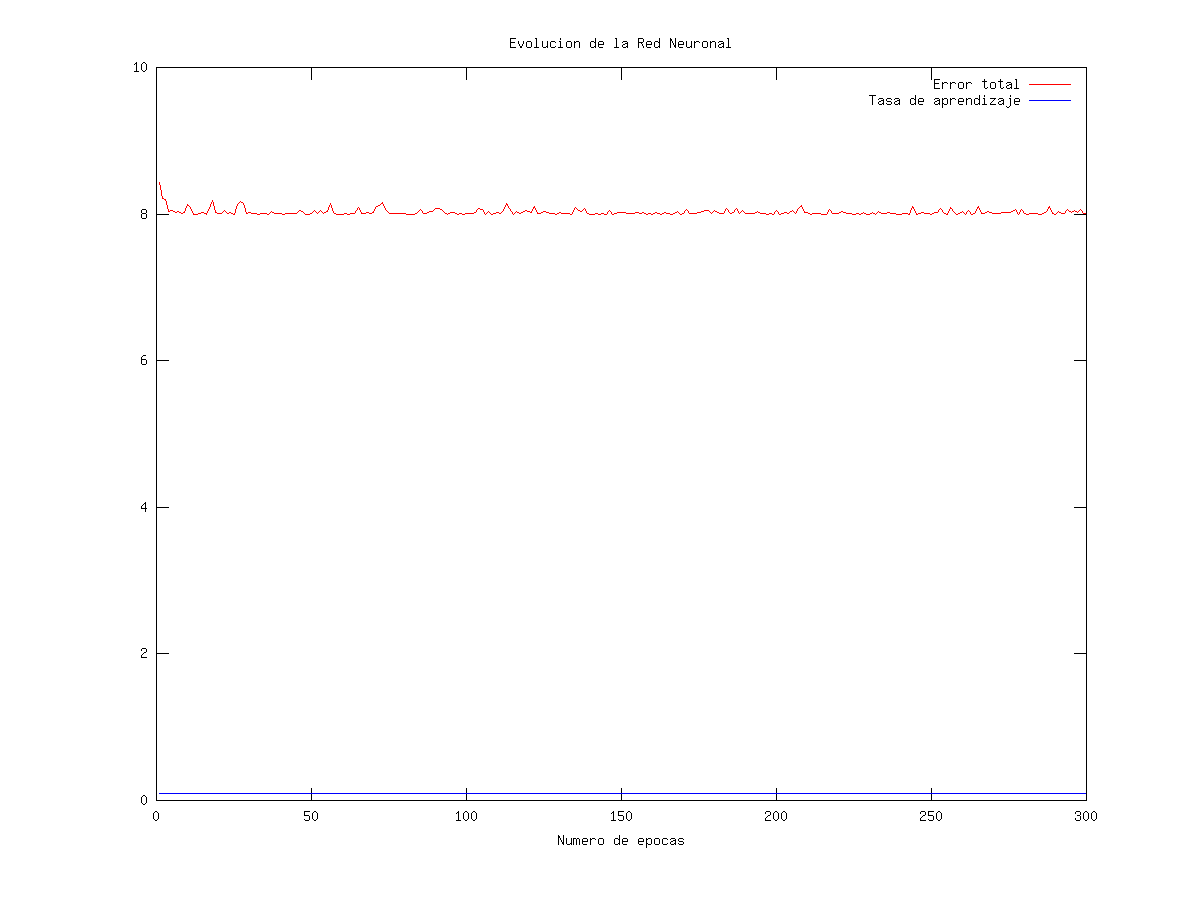
\includegraphics[scale=0.30]{./images/LinearConstante.png}
\label{modelado}
\end{center}
\end{figure}

\begin{center}
\par Figura 1: Ejemplo de estancamiento en mínimo local debido a la utilización de una función de transferencia lineal.
\end{center}

\begin{figure}[H]
\begin{center}
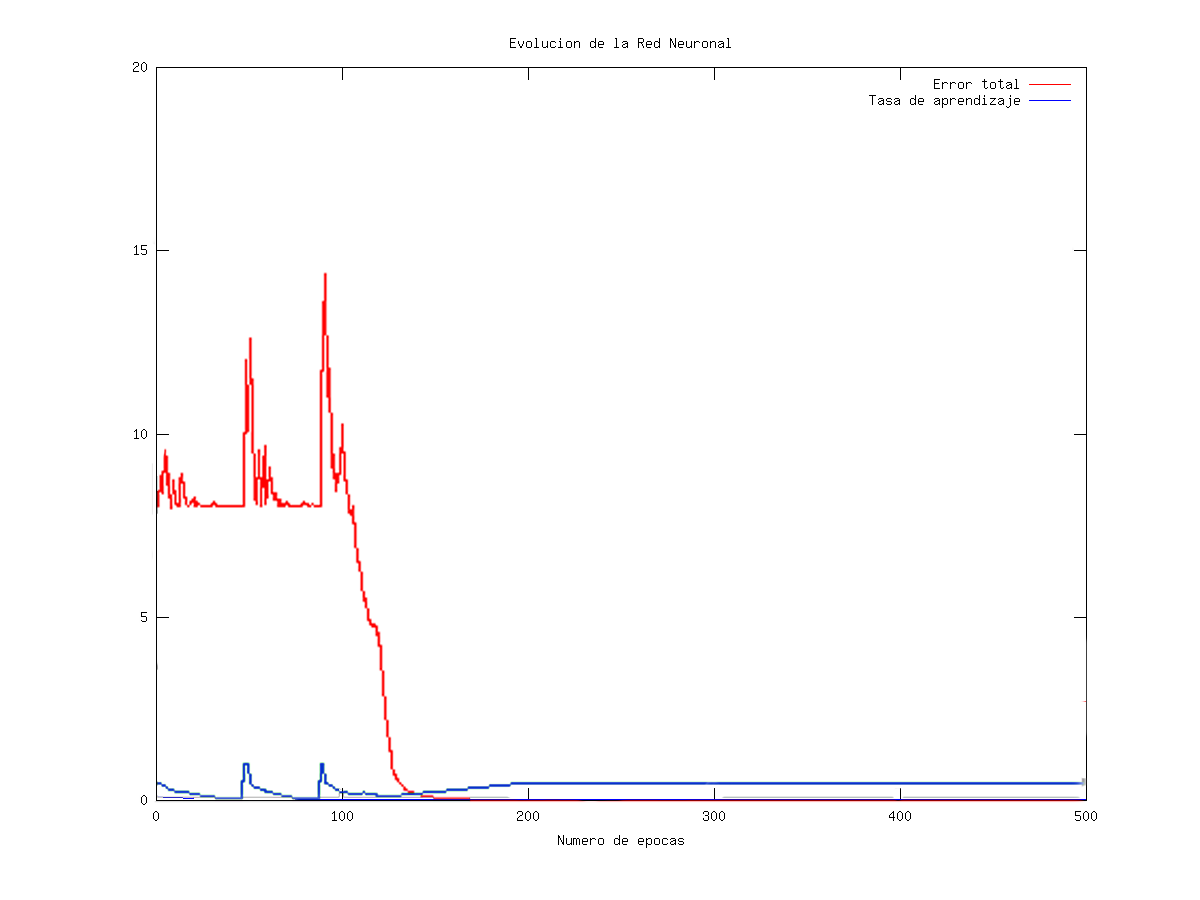
\includegraphics[scale=0.30]{./images/escapeminlocal.png}
\label{modelado}
\end{center}
\end{figure}

\begin{center}
\par Figura 2: Escape de mínimo local utilizando eta dinámico para el problema de paridad de 3 bits usando 500 épocas y una arquitectura de una capa oculta con 3 neuronas.
\end{center}

\clearpage

\begin{figure}[H]
\begin{center}
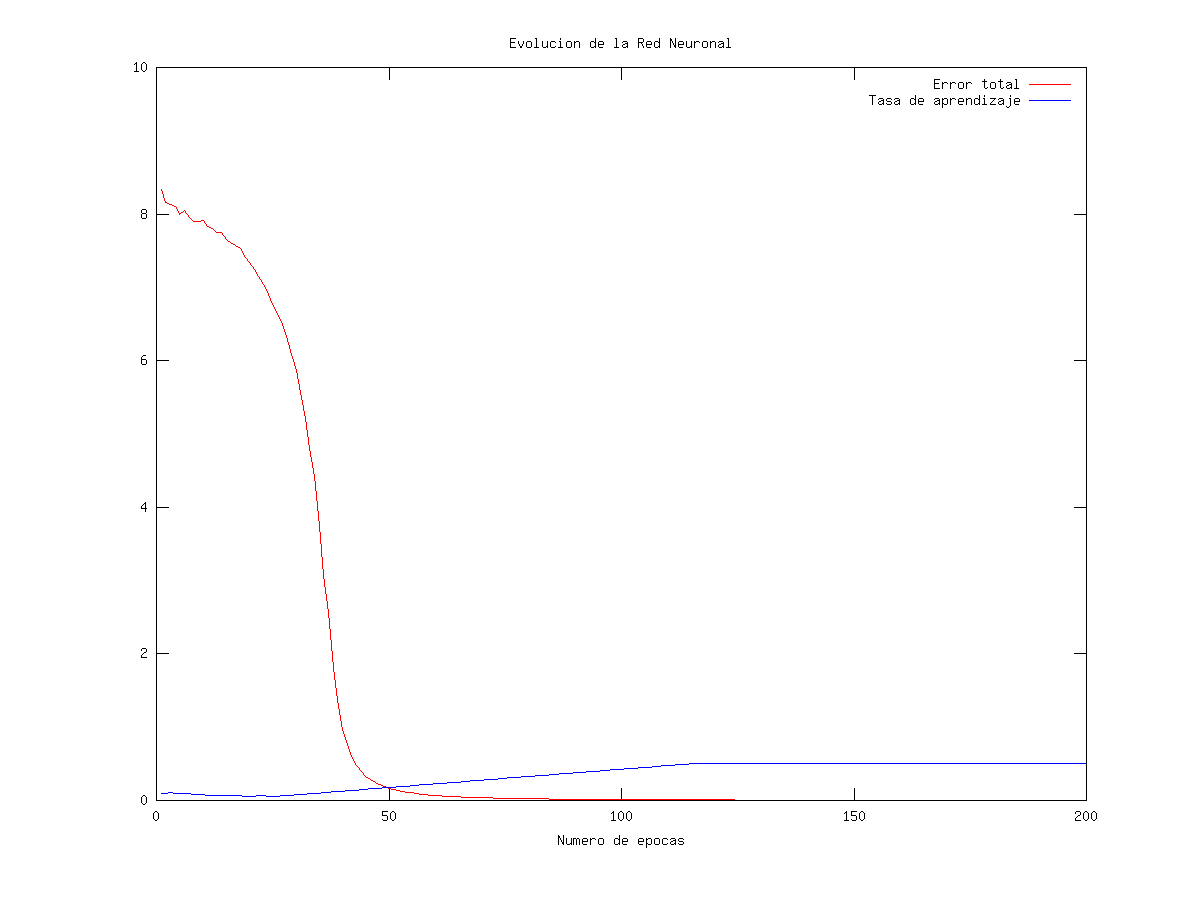
\includegraphics[scale=0.30]{./images/incremento.png}
\label{modelado}
\end{center}
\end{figure}

\begin{center}
\par Figura 3: Muestra cómo se incrementa hasta el valor máximo eta cuando la red neuronal resuelve el problema con el error deseado.
\end{center}




%\VerbatimInput{./code/calculoAb.m}




\end{document}